\documentclass[12pt,a4paper]{article}

% Paquetes básicos
\usepackage[utf8]{inputenc}
\usepackage[spanish]{babel}
\usepackage{graphicx}
\usepackage{xcolor}
\usepackage{amsmath}
\usepackage{amssymb}
\usepackage{hyperref}
\usepackage{geometry}
\usepackage{listings}
\usepackage{xcolor}
\usepackage{float}
\usepackage{epigraph}
\usepackage{cite}
\usepackage{listings}
\usepackage[listings]{tcolorbox}
\tcbuselibrary{listings, skins, breakable}
\lstloadlanguages{SQL}
\usepackage{xcolor}
\usepackage{subcaption}
\usepackage{url}

% Configurar márgenes
\geometry{
    top=2cm,
    bottom=2cm,
    left=2cm,
    right=2cm
}

% Configurar listings
\lstset{
    basicstyle=\small\ttfamily,
    breaklines=true,
    frame=single,
    numbers=left,
    numberstyle=\tiny,
    captionpos=b
}

% Información del documento
\title{\textsc{Entrega 3: ADE \& MongoDB}}
\author{Marcelo Ferreiro Sánchez, Pablo Chantada Saborido\\  Gillermo García Engelmo \& Pepe Romero Conde}
\date{\today}


\lstdefinelanguage{SQL}{
  morekeywords={
    SELECT,FROM,WHERE,AND,OR,INSERT,INTO,VALUES,UPDATE,SET,DELETE,CREATE,TABLE,
    ALTER,DROP,JOIN,INNER,LEFT,RIGHT,FULL,ON,AS,ORDER,BY,GROUP,HAVING,DESC,ASC,
    DISTINCT,COUNT,SUM,AVG,MIN,MAX,IN,IS,NOT,NULL,LIKE,BETWEEN,EXISTS,UNION
  },
  sensitive=false,
  morecomment=[l]{--},
  morecomment=[s]{/*}{*/},
  morestring=[b]',
  morestring=[b]"
}

\definecolor{azulito}{RGB}{186,200,211}
\definecolor{azul_oscuro}{RGB}{35,68,93}
\definecolor{turquesa}{RGB}{174,143,171}

\lstset{
  language=SQL,
  basicstyle=\color{azul_oscuro}\ttfamily\small,
  keywordstyle=\color{white}\bfseries,
  commentstyle=\color{gray}\itshape,
  stringstyle=\color{turquesa},
  backgroundcolor=\color{azulito},
  frame=single,
  numbers=left,
  numberstyle=\tiny\color{gray},
  breaklines=true,
  tabsize=2
}


\begin{document}

\maketitle

\tableofcontents

\newpage

\section{Introdución}

Como nas prácticas anteriores, traballamos sobre o conxunto de datos de AirB\&B. Neste caso truncamos o punto de vista ou a aplicación. Se ben anteriormente o foco era na explotación analítica de o feito \texttt{valoración} agora centrámosnos nos \texttt{hospedaxes}. O diseño da Base de datos terá lugar na sección \ref{sec:deseño}, e será realizado sobre os datos expostos en \ref{sec:modeloDatos}.

\section{Modelo de Datos}
\label{sec:modeloDatos}

Nesta ocasión non nos limitamos a usar os \texttt{.csv}s de unha cidade, con motivo de enriquezer as estadísticas. Dende un principio observamos que o porcentaxe de nulos non era ó meso ó longo das cidades, por eso con varias cidades esperamos unha respresentación máis fiel da realidade. As primeiras manipulacións que  tivemos que facerlle ós datos foi a de eliminar as columnas que non nos interesasen, engadir a columna de ``cidade'' e apilar todo nun \texttt{csv}. Fixemos ese traballo ca librería Pandas de Python (ver \texttt{sripts/clean\_csvs.py}).  

As columnas elexidas \textcolor{red}{[FALAR DAS COLUMNAS ELIXIDAS, A ELECCION]}

As cidades elixidas foron: Barcelona, Euskadi, Girona, Lisboa, Madrid, Malaga, Mallora, Menorca, Porto, Sevilla e Valencia. O Modelo de Datos co porcentaxe de nulos reportado para estas cidades pode verse na figura \ref{fig:modeloDatos}.



\begin{figure}[H]
    \centering
    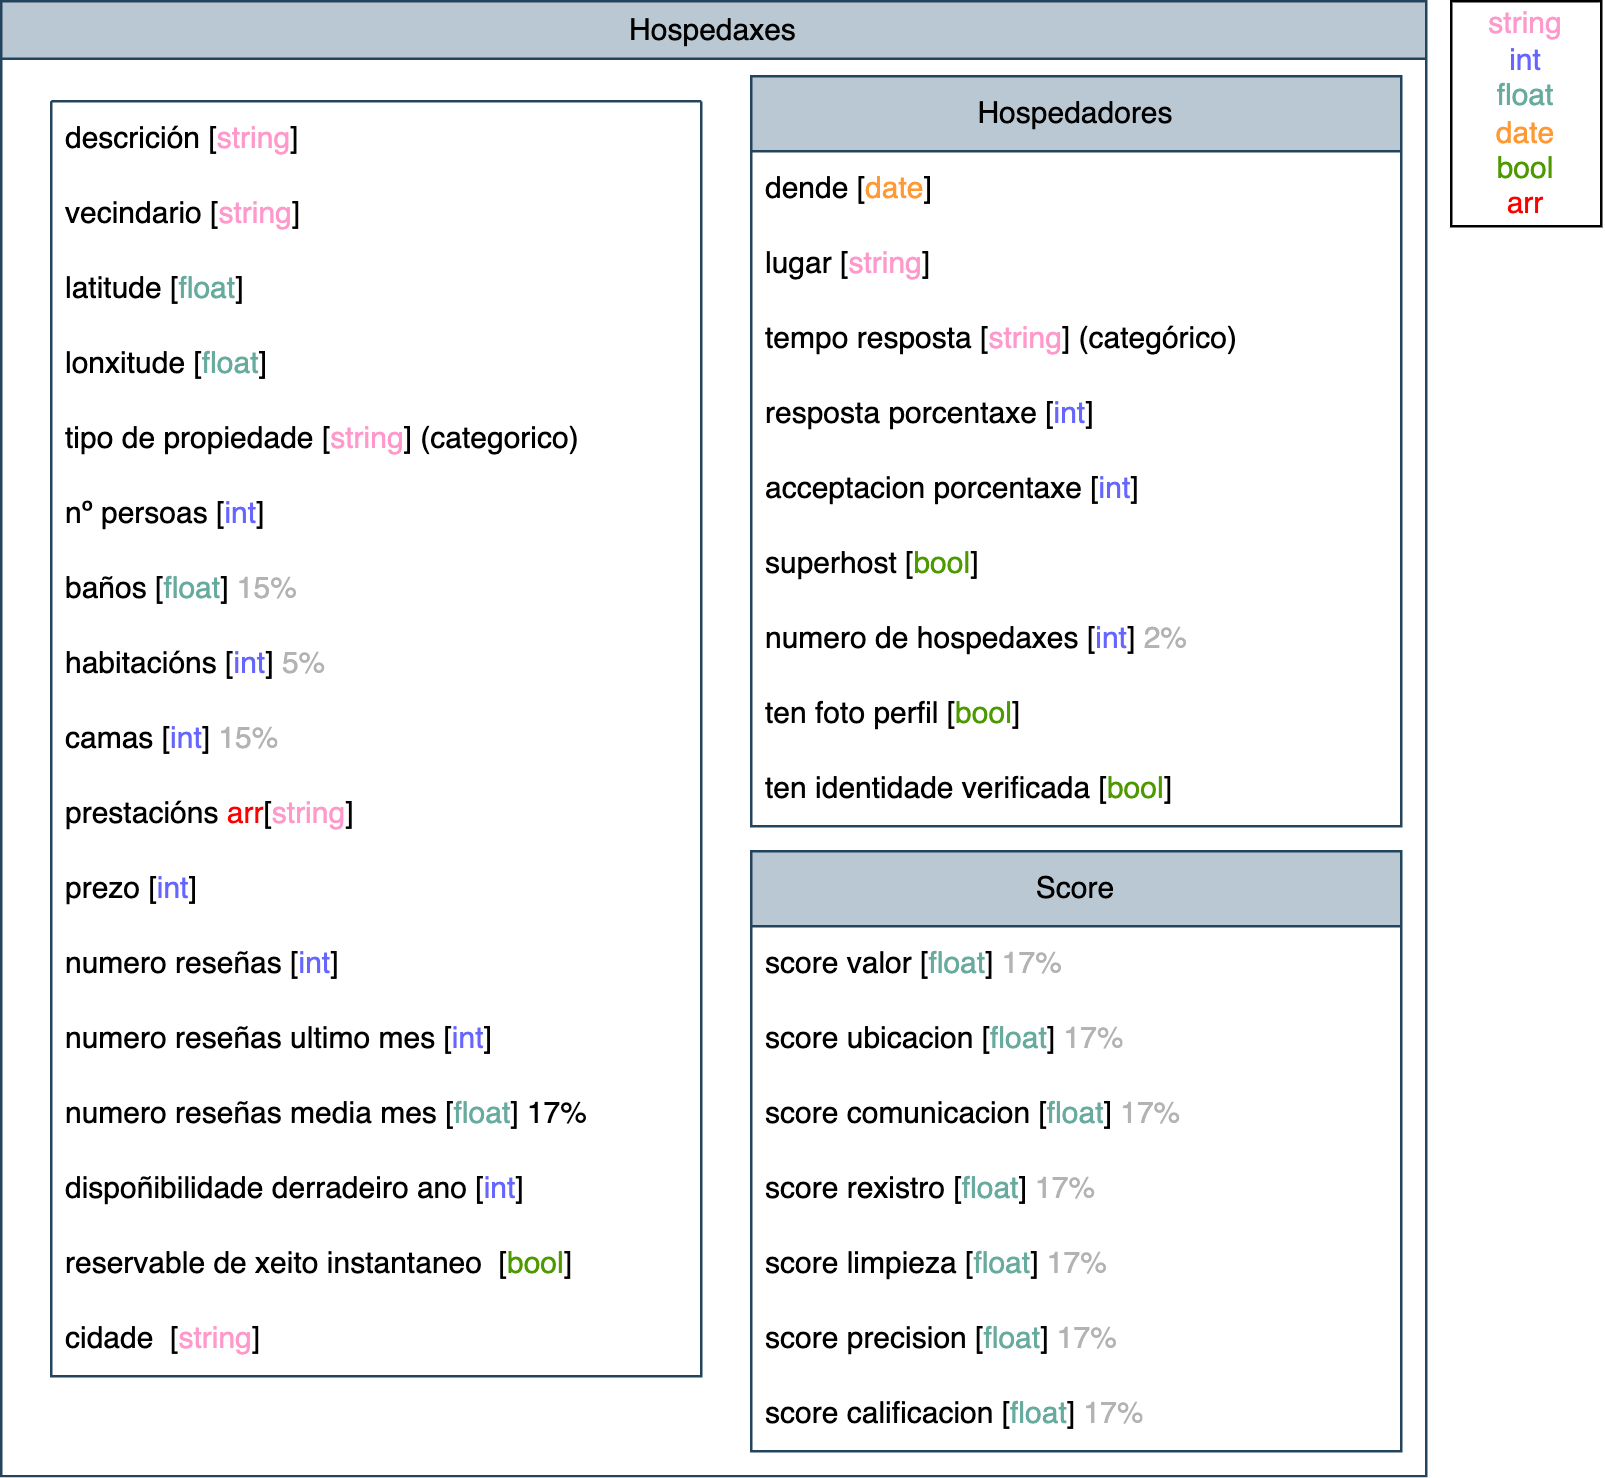
\includegraphics[width=1\textwidth]{../diagramas/modeloDatos.drawio.png}
    \caption{Diagrama do Modelo de Datos}
  \label{fig:modeloDatos}
\end{figure}

\section{Preprocesado de datos}

\textcolor{red}{
\begin{itemize}
	\item Análisis exploratorio inicial. Mostrar forma y tamaño del dataset, identificar tipos de datos,
	identificar valores nulos y detectar posibles outliers.
	\item Tratamiento de valores faltantes. Aplicar al menos dos estrategias diferentes, justificadas según
	el tipo de variable: eliminar registros con demasiados nulos, rellenar variables numéricas (media,
	mediana, etc.), rellenar categóricos (utilizando la moda o una categoría especial), sustituir
	mediante reglas específicas del dominio.
\item Transformaciones adicionales. Según proceda en el dominio, deben aplicarse al menos dos
	transformaciones tales como:
		\subitem Normalización o estandarización de variables numéricas.
		\subitem Codificación simple de valores categóricos.
		\subitem Limpieza de texto simple (trim, lowercase, …).
		\subitem Agrupaciones o reducción de categorías (por ejemplo, High, Medium, Low).
	\item Balanceo de datos. Si el dominio lo requiere deben aplicarse técnicas de undersampling,
oversampling, filtrado de ruido, etc. (Opcional, solo si es pertinente en caso de hacer tarea 4)
\end{itemize}
}

\subsection{Análisis exploratorio del dataset}
\subsection{Tratamiento de nulos}

En canto o tratamento de nulos, dicir que todos son de tipo númerico. Isto condiciona as opcións de imputación. Ademáis pódense que os nulos divídense en tres grupos: os relacionados co inmobiliario (baños, habitacións e camas), os valores de \epmh{Score} e o número de hospedaxes. Unha primera idea de encher os nulos dun grupo con valores do mesmo (e.g. imputar o \emph{score} de comunicación co resto de \emph{scores}) desmantelouse á vista da Figura \ref{fig:nulos}



\begin{figure}[H]
    \centering
    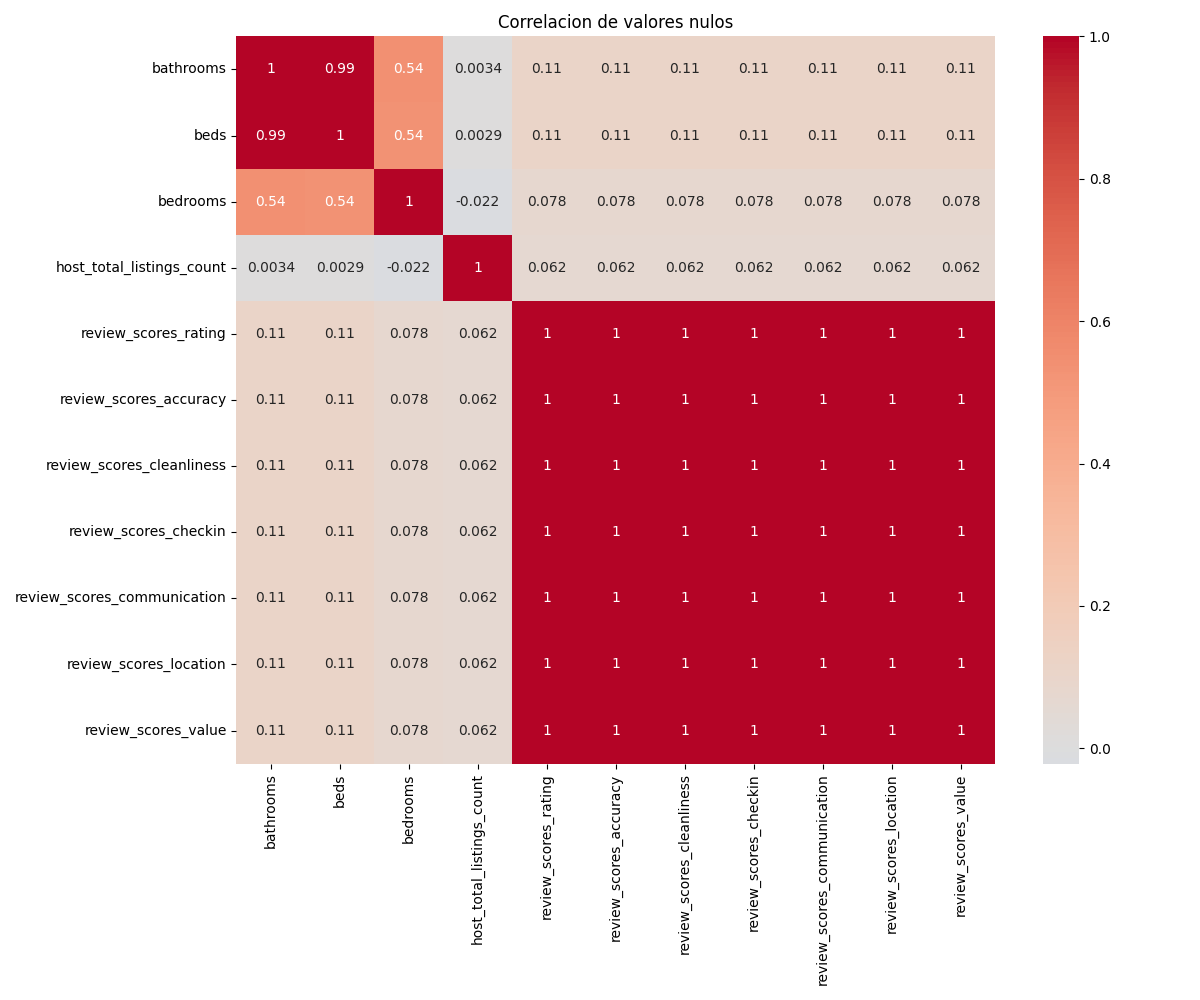
\includegraphics[width=1\textwidth]{../diagramas/null_correlation_heatmap.png}
    \caption{Correlación entre os nulos. Pódese apreciar claramente que os \emph{scores} son nulos á vez, igual que cos membros do inmobiliario.}
  \label{fig:nulos}
\end{figure}

\begin{figure}[H]
    \centering
    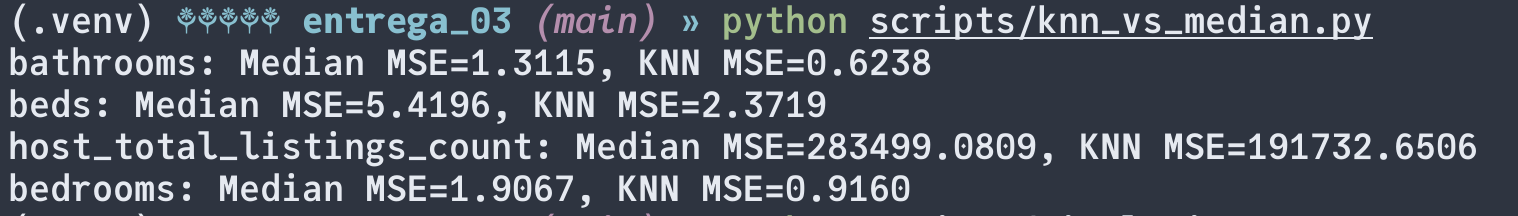
\includegraphics[width=1\textwidth]{../diagramas/vale_pena_Knn.png}
    \caption{Comparación dos métodos de imputación KNN ($k$=3) e mediana sobre a métrica $\mathcal{L}_2$. Os resultados repórtanse con KFold de $k$=2.}
  \label{fig:vale_pena_Knn}
\end{figure}

\subsection{Otras operaciones de procesado}

\section{Definición e implementación de la Base de Datos}
\label{sec:deseño}

\textcolor{red}{
	\begin{itemize}
		\item Deberá crearse una base de datos específica para el dominio en una instalación propia de
MongoDB, en la que se importarán los datos usando una de las tres formas:
\subitem Pymongo para importación directa desde Python.
\subitem Exportación en formato JSON y carga mediante MongoDB Compass.
\subitem Exportación en formato JSON e importación mediante mongoimport desde terminal.
\item Explicar detalladamente la estructura de los documentos (anidar objetos, arrays, decisiones de
normalización o desnormalización). Justificar el modelo elegido y posibles alternativas.
	\end{itemize}
}

\section{Explotación de la Base de Datos}
\textcolor{red}{Cada grupo deberá implementar 4 consultas que respondan a preguntas analíticas relevantes dentro de su
dominio. Se valorará positivamente el uso del pipeline de agregación.
Algunos ejemplos de categorías válidas serían: cálculo de estadísticas numéricas, agrupaciones por barrio/tipo
de habitación/host/país, ranking (top de precios/valoraciones), detección de anomalías o valores extremos,
evolución temporal.
Cada consulta debe incluir:
\begin{itemize}
	\item Enunciado claro de la pregunta analítica que quiere responder.
	\item Consulta completa o pipeline en sintaxis MongoDB.
\item Resultados resumidos o capturas de la salida, acompañados de una breve explicación de la salida.
\end{itemize}}
Agora que hemos definido e implementado a nosa Base de Datos, 

\subsection*{Consulta 1: Obter un índice de centralidade (dentro da cidade) para cada hospedaxe} 
\addcontentsline{toc}{subsection}{Consulta 1}

\emph{Justificación:}

\emph{Resultados:}

\begin{lstlisting}
SELECT
\end{lstlisting}

\subsection*{Consulta 2: Cales son os barrios con hospedadores máis novos? Para cada cidade} 
\addcontentsline{toc}{subsection}{Consulta 2}

\emph{Justificación:}

\emph{Resultados:}

\begin{lstlisting}
SELECT
\end{lstlisting}

\subsection*{Consulta 3: Influe foto de perfil no prezo medio?} 
\addcontentsline{toc}{subsection}{Consulta 3}

\emph{Justificación:}

\emph{Resultados:}

\begin{lstlisting}
SELECT
\end{lstlisting}

\subsection*{Consulta 4: Cales son os barrios con hospedaxes máis grandes (máis habitacións)?} 
\addcontentsline{toc}{subsection}{Consulta 4}

\emph{Justificación:}

\emph{Resultados:}

\begin{lstlisting}
SELECT
\end{lstlisting}


\subsection*{Consulta 5: Que \epmh{score} é o que máis fluctua?} 
\addcontentsline{toc}{subsection}{Consulta 5}

\emph{Justificación:}

\emph{Resultados:}

\begin{lstlisting}
SELECT
\end{lstlisting}

\subsection*{Consulta 6: Cales son os hospedaxes con hospedadores fóra desa cidade?}
\addcontentsline{toc}{subsection}{Consulta 6}

\emph{Justificación:}

\emph{Resultados:}

\begin{lstlisting}
SELECT
\end{lstlisting}

\subsection*{Consulta 7: Cales son os hospedaxes que estan a facer un bo último mes?}
\addcontentsline{toc}{subsection}{Consulta 7}

\emph{Justificación:}

\emph{Resultados:}

\begin{lstlisting}
SELECT
\end{lstlisting}

\section{Recheo de nulos usando Aprendizaxe Automático}
\textcolor{red}{De forma opcional y rápida, entrenar un modelo de aprendizaje automático utilizando los datos almacenados
en MongoDB (por ejemplo, regresión, clasificación, …). Debe explicarse brevemente el objetivo del modelo,
las variables utilizadas y los resultados principales.}

Como a columna \texttt{price} nos \texttt{.csv}s orixinais tiña un 10\% de nulos, decidimos  entrenar un modelo de Aprendizaxe Automático para \emph{regresar} los valores de precio. Ademáis, esta tarea parecíanos interesante de por sí.

\newpage

\bibliographystyle{IEEEtran}
\bibliography{referencias}


\end{document}

